\section{Modelo de Domínio e Dados}

\subsection{Entidades no Modelo Conceptual}
\subsubsection{users}
\begin{itemize}
  \item \texttt{id (bigserial)} — identificador único do utilizador.
  \item \texttt{email (varchar)} — email de autenticação (valor único).
  \item \texttt{password (varchar)} — hash seguro da palavra-passe.
  \item \texttt{role (boolean)} — papel do utilizador (admin=true, user=false).
  \item \texttt{created\_at (timestamp)} — data/hora de criação do registo.
\end{itemize}

\subsubsection{scenarios}
\begin{itemize}
  \item \texttt{id (bigserial)} — identificador do cenário.
  \item \texttt{name (text)} — nome curto único do cenário.
  \item \texttt{description (text)} — descrição do cenário.
  \item \texttt{is\_builtin (boolean)} — indica se é um cenário pré-instalado.
  \item \texttt{storage\_path (text)} — caminho do ficheiro do cenário.
  \item \texttt{created\_at (timestamp)} — data/hora de criação do registo.
\end{itemize}

\subsubsection{template\_datasets}
\begin{itemize}
  \item \texttt{id (bigserial)} — identificador do dataset.
  \item \texttt{name (text)} — nome do dataset.
  \item \texttt{description (text)} — descrição/resumo do dataset.
  \item \texttt{storage\_path (text)} — caminho do ficheiro do dataset.
  \item \texttt{is\_builtin (boolean)} — indica se é um dataset pré-instalado.
  \item \texttt{created\_at (timestamp)} — data/hora de criação do registo.
\end{itemize}

\subsubsection{role\_play\_options}
\begin{itemize}
  \item \texttt{id (bigserial)} — identificador da opção de role play.
  \item \texttt{name (text)} — nome da opção de role play.
  \item \texttt{description (text)} — descrição da opção.
  \item \texttt{is\_builtin (boolean)} — indica se é uma opção pré-instalada.
  \item \texttt{storage\_path (text)} — caminho do ficheiro da opção.
  \item \texttt{created\_at (timestamp)} — data/hora de criação do registo.
\end{itemize}

\subsubsection{models}
\begin{itemize}
  \item \texttt{name (text)} — identificador único do modelo (ex.: \texttt{llama3.1:8b}).
\end{itemize}

\subsubsection{runs\_metrics}
\begin{itemize}
  \item \texttt{id (bigserial)} — identificador da execução (run).
  \item \texttt{target\_model (text)} — nome do modelo alvo.
  \item \texttt{attack\_model (text)} — nome do modelo atacante (quando aplicável).
  \item \texttt{visibility (text)} — visibilidade dos resultados.
  \item \texttt{role\_play\_option\_id (bigint)} — FK para a opção de role play usada.
  \item \texttt{attack\_type (varchar)} — tipo de ataque usado.
  \item \texttt{status (char)} — estado da execução (\texttt{queued|running|judging|done|failed}).
  \item \texttt{langfuse\_trace\_id (text)} — identificador do trace correspondente no Langfuse.
  \item \texttt{started\_at (timestamp)} — data/hora de início da execução.
  \item \texttt{ended\_at (timestamp)} — data/hora de fim da execução.
  \item \texttt{metrics\_asr (float)} — \textit{Attack Success Rate} da execução.
  \item \texttt{metrics\_orr (float)} — \textit{Over-Refusal Rate} da execução.
  \item \texttt{metrics\_aor (float)} — \textit{Achieved Objective Rate} da execução.
  \item \texttt{static\_metric (float)} — métrica estática da execução.
  \item \texttt{metrics\_veridict\_majority (boolean)} — consenso final sobre o veredito do ataque.
  \item \texttt{template\_datasets\_id (bigint)} — FK para o dataset usado.
  \item \texttt{scenarios\_id (bigint)} — FK para o cenário usado.
  \item \texttt{users\_id (bigint)} — FK para o utilizador dono da execução.
\end{itemize}

\subsubsection{jury\_votes}
\begin{itemize}
  \item \texttt{id (bigserial)} — identificador do voto do jurado.
  \item \texttt{jury\_index (smallint)} — posição do jurado na votação.
  \item \texttt{usefulness (boolean)} — utilidade atribuída à resposta do modelo alvo.
  \item \texttt{veridict (boolean)} — decisão do jurado em relação à conformidade/segurança da resposta.
  \item \texttt{model\_name (text)} — nome do modelo do jurado.
  \item \texttt{created\_at (timestamp)} — data/hora de criação do registo.
  \item \texttt{runs\_metrics\_id (bigint)} — FK para a execução avaliada.
\end{itemize}

\subsubsection{api\_key\_configs}
\begin{itemize}
  \item \texttt{id (serial)} — identificador da configuração de API key.
  \item \texttt{name (varchar)} — nome da configuração.
  \item \texttt{provider (varchar)} — fornecedor da API (default: OPEN\_AI).
  \item \texttt{model\_name (varchar)} — nome do modelo associado.
  \item \texttt{api\_key (varchar)} — chave de API.
  \item \texttt{user\_id (bigint)} — FK para o utilizador dono da configuração.
\end{itemize}

\subsubsection{audit\_logs}
\begin{itemize}
  \item \texttt{id (bigserial)} — identificador do log de auditoria.
  \item \texttt{user\_id (bigint)} — FK para o utilizador que fez a ação.
  \item \texttt{endpoint (varchar)} — endpoint acedido.
  \item \texttt{request\_body (jsonb)} — corpo do pedido.
  \item \texttt{created\_at (timestamp)} — data/hora de criação do registo.
\end{itemize}

\subsection{Relações entre Entidades}
Na Figura \ref{fig:diagrama_database_relacoes} podemos observar as relações entre as entidades na base de dados.
\begin{figure}[H]
  \centering
  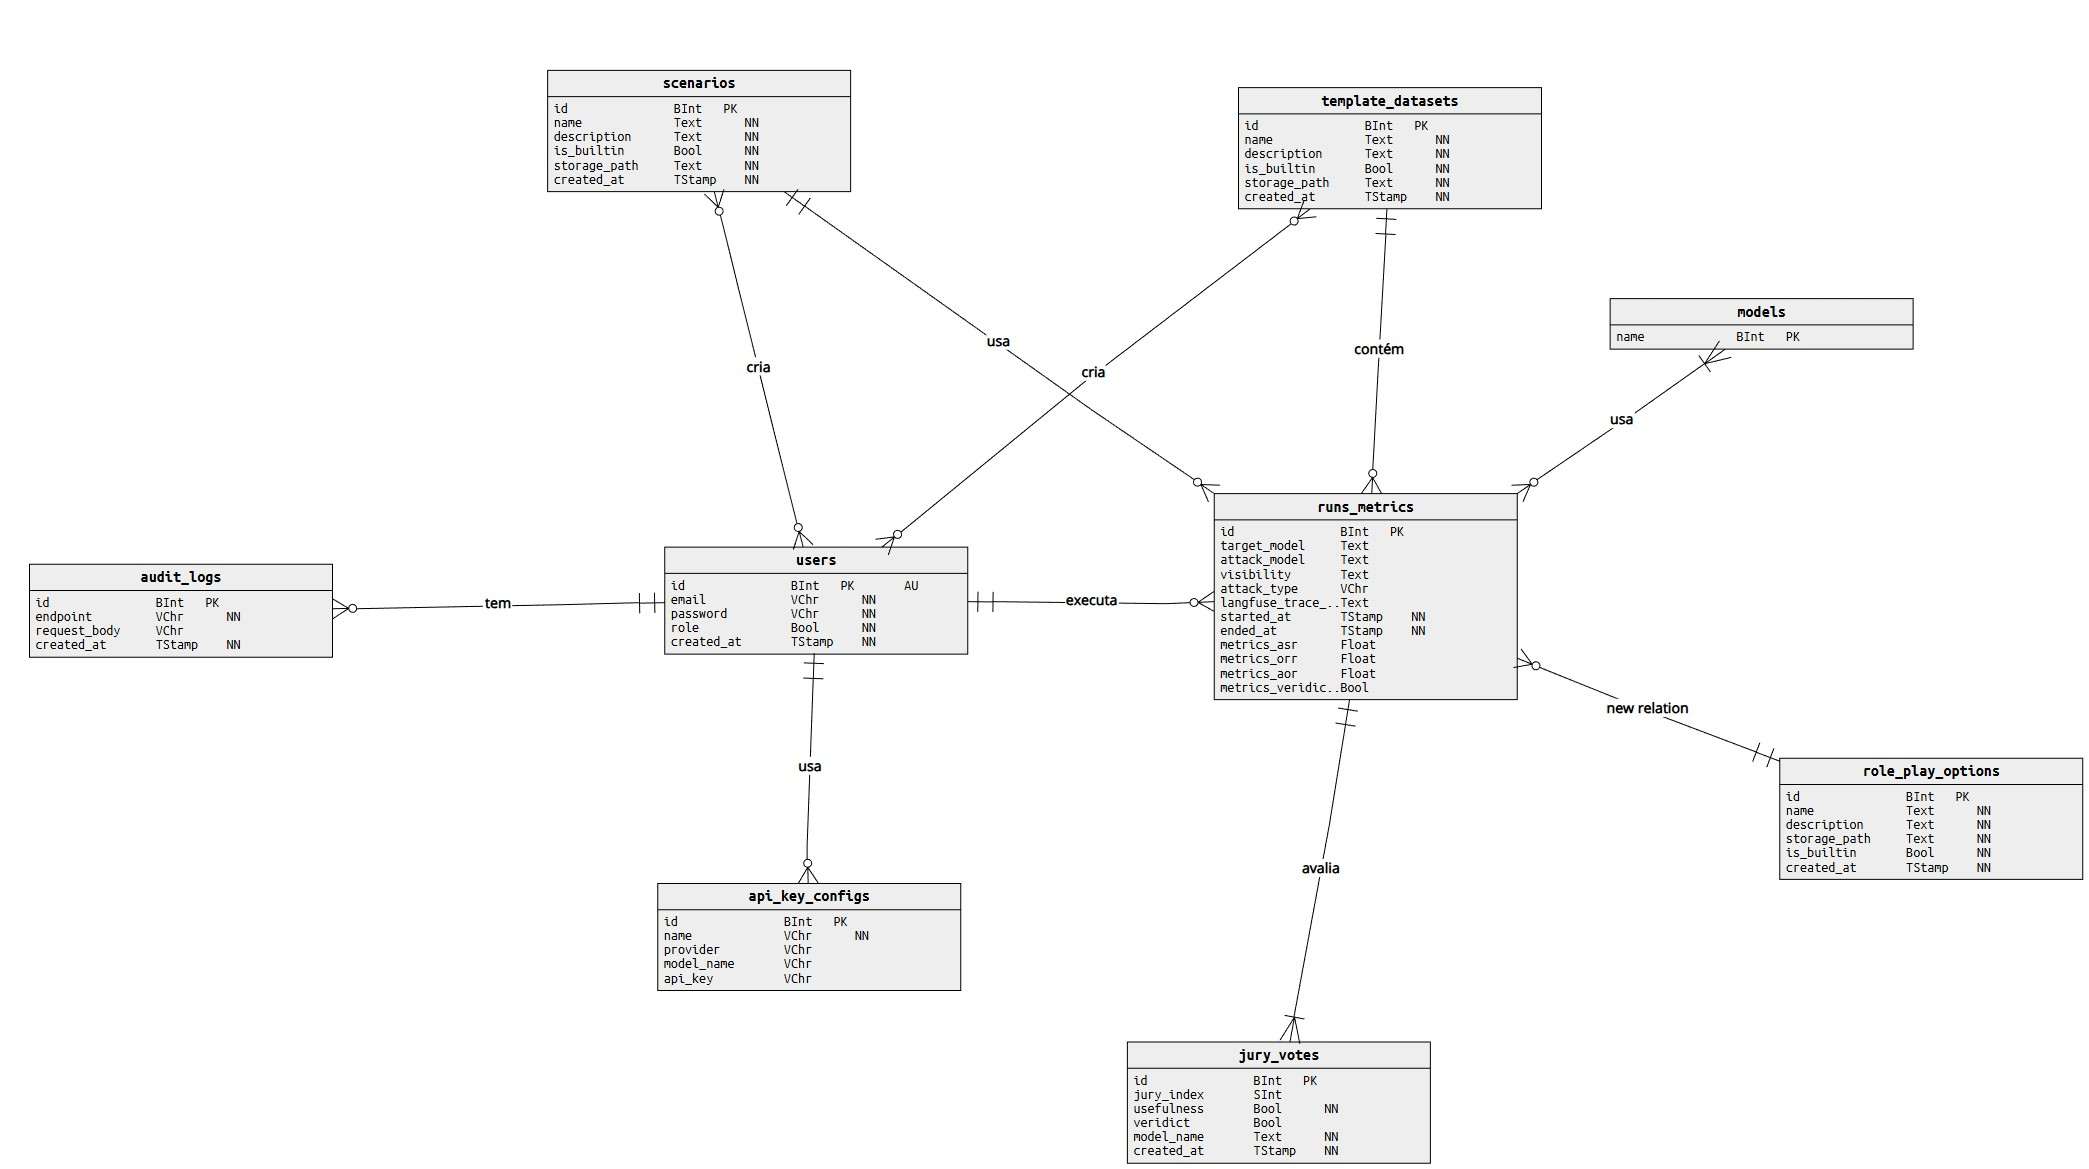
\includegraphics[width=\linewidth]{images/database_relations.jpeg}
  \caption{Relações entre as entidades da base de dados}
  \label{fig:diagrama_database_relacoes}
\end{figure}

